\documentclass{beamer}
\usepackage[latin1]{inputenc}

\usetheme{Madrid}
\usecolortheme{default}
\usepackage{amsmath}
\usepackage{amssymb,amsfonts,amsthm}
\usepackage{txfonts}
\usepackage{tkz-euclide}
\usepackage{listings}
\usepackage{adjustbox}
\usepackage{array}
\usepackage{tabularx}
\usepackage{gvv}
\usepackage{lmodern}
\usepackage{circuitikz}
\usepackage{tikz}
\usepackage{graphicx}
\usepackage{gensymb}
\usepackage{physics}

\setbeamertemplate{page number in head/foot}[totalframenumber]

\usepackage{tcolorbox}
\tcbuselibrary{minted,breakable,xparse,skins}



\definecolor{bg}{gray}{0.95}
\DeclareTCBListing{mintedbox}{O{}m!O{}}{%
  breakable=true,
  listing engine=minted,
  listing only,
  minted language=#2,
  minted style=default,
  minted options={%
    linenos,
    gobble=0,
    breaklines=true,
    breakafter=,,
    fontsize=\small,
    numbersep=8pt,
    #1},
  boxsep=0pt,
  left skip=0pt,
  right skip=0pt,
  left=25pt,
  right=0pt,
  top=3pt,
  bottom=3pt,
  arc=5pt,
  leftrule=0pt,
  rightrule=0pt,
  bottomrule=2pt,
  toprule=2pt,
  colback=bg,
  colframe=orange!70,
  enhanced,
  overlay={%
    \begin{tcbclipinterior}
    \fill[orange!20!white] (frame.south west) rectangle ([xshift=20pt]frame.north west);
    \end{tcbclipinterior}},
  #3,
}
\lstset{
    language=C,
    basicstyle=\ttfamily\small,
    keywordstyle=\color{blue},
    stringstyle=\color{orange},
    commentstyle=\color{green!60!black},
    numbers=left,
    numberstyle=\tiny\color{gray},
    breaklines=true,
    showstringspaces=false,
}
\title{8.4.28}
\date{10th october, 2025}
\author{Vishwambhar - EE25BTECH11025}

\begin{document}

\frame{\titlepage}
\begin{frame}{Question}
The axis of the parabola is along the line $y=x$ and trhe distance of its vertex and focus from origin are $\sqrt{2}$ and $2\sqrt{2}$ respectively. If the vertex and focus both lie in the first quadrant, then the equation of the parabola is
\begin{enumerate}
\begin{multicols}{2}
    \item $(x+y)^2=(x-y-2)$
    \item $(x-y)^2=(x+y-2)$
    \item $(x-y)^2=4(x+y-2)$
    \item $(x-y)^2=8(x+y-2)$
\end{multicols}
\end{enumerate}\end{frame}

\begin{frame}{Let}
Let:\\
Focus of the parabola be $\vec{F}$\\
Vertex of the parabola be $\vec{V}$\\
Normal vector to the directrix be $\vec{n}$\\
The point of intersection of directrix and axis be $\vec{P}$\\
Direction vector and slope of axis be $\vec{m}_1$ and $m_1$\\
Direction vector and slope of directrix be $\vec{m}_2$ and $m_2$\\
Equation of axis be $\vec{x}=\lambda\vec{m}_1$\\
\end{frame}

\begin{frame}{Given}
Given:
\begin{align}
    \norm{\vec{F}} = 2\sqrt{2}\\
    \norm{\vec{V}} = \sqrt{2}\\
    \vec{m}_1 = \myvec{1\\m_1}=\myvec{1\\1}
\end{align}
\end{frame}

\begin{frame}{Focus, Vertex}
Finding focus($\vec{F}$):
\begin{align}
    \lambda\vec{m}_1=\vec{F}\\
    \lambda = \pm\frac{\norm{\vec{F}}}{\norm{\vec{m}_1}}\\
    \vec{F} = \pm\frac{\norm{\vec{F}}}{\norm{\vec{m}_1}}\vec{m}_1
\end{align}

Finding vertex($\vec{V}$)
\begin{align}
    \lambda\vec{m}_1=\vec{V}\\
    \lambda = \pm\frac{\norm{\vec{V}}}{\norm{\vec{m}_1}}\\
    \vec{V} = \pm\frac{\norm{\vec{V}}}{\norm{\vec{m}_1}}\vec{m}_1
\end{align}
\end{frame}

\begin{frame}{Directrix}
Since directrix will be perpendicular to axis $m_1m_2=-1$
\begin{align}
    \vec{m_2} = \myvec{1\\m_2} = \myvec{1\\ \frac{-1}{m_1}}\\
    \vec{n} = \myvec{0&1\\-1&0}\vec{m_2}
\end{align}

Since $\vec{V}$ will be midpoint of $\vec{P}$ and $\vec{F}$ and also $\vec{P}$:
\begin{align}
    \frac{\vec{P}+\vec{F}}{2} = \vec{V}\\
    \vec{P}=2\vec{V}-\vec{F}
\end{align}
\end{frame}

\begin{frame}{Parabola}
Now, finding the directrix equation in normal form;
\begin{align}
    \vec{n}^\top\vec{x}=\vec{n}^\top\vec{P}
\end{align}

From equation of conic $\vec{x}^\top A\vec{x}+2\vec{u}^\top\vec{x}+f=0$\\
For parabola:
\begin{align}
    A=\norm{\vec{n}}^2I-\vec{n}\vec{n}^\top\\
    \vec{u}=c\vec{n}-\norm{\vec{n}}^2\vec{F}=\vec{n}^2\vec{P}\vec{n}-\norm{\vec{n}}^2\frac{\norm{\vec{F}}}{\norm{\vec{m}_1}}\vec{m}_1\\
    f=\norm{\vec{n}}^2\norm{\vec{F}}^2-c^2=\norm{\vec{n}}^2\norm{\vec{F}}^2-\brak{\vec{n}^\top\vec{P}}^2
\end{align}

\end{frame}

\begin{frame}{Conclusion}
Substituting values given in question we get:
\begin{align}
    A=\myvec{1&-1\\-1&1}\\
    \vec{u}=-4\myvec{1\\1}\\
    f=16
\end{align}

Substituting (18), (19) and (20) in conic equation we get:
\begin{align}
    \myvec{x&y}\myvec{1&-1\\-1&1}\myvec{x\\y}+\brak{-4}\myvec{1&1}\myvec{x\\y}+16=0\\
    \brak{x+y}^2=8\brak{x+y-2}
\end{align}
Hnece, option(4) is correct.
\end{frame}


\begin{frame}[fragile]
    \frametitle{C Code}
    \begin{lstlisting}
 #include<stdio.h>
 #include<math.h>

 double normf;
 double normv;
 double dvectora[2] = {1,1};
 double m1 = 1;

 double norm(double arr1[2]){
    double sum = 0;
    for(int i = 0; i<2; i++){
        sum+=(sqrt(arr1[i]*arr1[i]));
    }
    return sum;
}
    \end{lstlisting}
\end{frame}

\begin{frame}[fragile]
    \frametitle{C code}
    \begin{lstlisting}
double vdotv(double arr1[2], double arr2[2]){
    double sum = 0;
    for(int i = 0; i<2; i++){
        sum+=(arr1[i]*arr2[i]);
    }
    return sum;
}
void vplusv(double t, double v1[2], double v2[2], double P[2]){
    if(t==1){
        for(int i = 0; i<2; i++){
            P[i]=v1[i]+v2[i];
        }
    }
    if(t==-1){
        for(int i = 0; i<2; i++){
            P[i]=v1[i]-v2[i];
        }
    }
}
    \end{lstlisting}
\end{frame}

\begin{frame}[fragile]
    \frametitle{C code}
    \begin{lstlisting}
void give_data(double *points){

    normf = 2*sqrt(2); normv = sqrt(2);
    double lambda;
    lambda =(normf/norm(dvectora));
    double vectorF[2];
    for(int i = 0; i<2; i++){
        vectorF[i] = lambda*dvectora[i];
    }
    lambda = (normv/norm(dvectora));
    double vectorV[2];
    for(int i = 0; i<2; i++){
        vectorV[i] = lambda*dvectora[i];
    }
    \end{lstlisting}
\end{frame}

\begin{frame}[fragile]
    \frametitle{C code}
    \begin{lstlisting}
    double m2 = -1/m1;
    double dvectorb[2] = {1, m2};
    double X[2] = {2*vectorV[0], 2*vectorV[1]};
    double P[2];
    vplusv(1, X, vectorF, P);
    double c;
    double n[2]={0};
    double imp[2][2] = {{0, 1},{-1, 0}};
    for(int i = 0; i<2; i++){
        for(int j = 0; j<2; j++){
            n[i]+=imp[i][j]*dvectora[j];}}
    c = vdotv(n, P);
     points[0] = -8;
     points[1] = -2;
     points[2] = 16;}
    \end{lstlisting}
\end{frame}

\begin{frame}[fragile]
    \frametitle{Python code 1}
    \begin{lstlisting}
import ctypes as ct

lib = ct.CDLL("./problem.so")

lib.give_data.argtypes = [ct.POINTER(ct.c_double)]

points = ct.c_double*3
data = points()
lib.give_data(data)

def send_data():
    return data[0], data[1], data[2]
    \end{lstlisting}
\end{frame}

\begin{frame}[fragile]
    \frametitle{Python code 2}
    \begin{lstlisting}
import matplotlib.pyplot as plt
import numpy as np
from call import send_data
a, b, c = send_data()
def parabola(x,y):
    return x**2+y**2+b*x*y+a*x+a*y+c
X, Y = np.meshgrid((np.linspace(-15, 15, 400)), (np.linspace(-15, 15, 400)))
Z = parabola(X,Y)
p = np.linspace(-10, 10, 200)
q = p
r = p = np.linspace(-10, 10, 200)
s = -r
    \end{lstlisting}
\end{frame}

\begin{frame}[fragile]
    \frametitle{Python code 2}
    \begin{lstlisting}
plt.plot(p,q,"-r")
plt.plot(r,s,"-g")
plt.plot(2,2,'ko')
plt.plot(1,1,'ko')
plt.contour(X,Y,Z,levels=[0], colors = "black", linewidths = 1)
plt.text(-6.5,-5.7,"y=x",color='black',fontsize = 12)
plt.text(-7.14,7.18,"y=-x", color = 'black', fontsize = 12)
plt.text(2.52, 11.64, r'$(x+y)^2=8(x+y-2)$', color = 'black', fontsize = 12)
plt.text(2.4,2,"(2,2)", color = 'black', fontsize = 10)
plt.text(1.05,0.65, "(1,1)", color = 'black', fontsize = 10)
    \end{lstlisting}
\end{frame}

\begin{frame}[fragile]
    \frametitle{Python code 2}
    \begin{lstlisting}
plt.xlabel("X-axis")
plt.ylabel("Y-axis")
plt.axvline(0, color='black', linewidth=2)
plt.axhline(0,color='black',linewidth=2)
plt.axis("equal")
plt.grid(True)
plt.show()
    \end{lstlisting}
\end{frame}

\begin{frame}{Plot}
    \begin{figure}
        \centering
        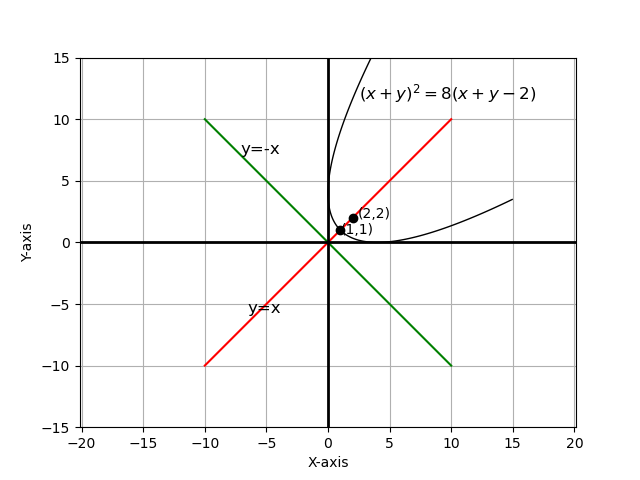
\includegraphics[width=0.5\columnwidth]{../figs/plot.png}
        \caption{Plot of the parabola}
        \label{fig:fig}
    \end{figure}
\end{frame}

\end{document}
